% The state of the dynamic program of Section 3: a set X of thresholds, and the sets X_1 and X_2
% that recursion (1) consults. Adapted from the slide "Dynamic Program".
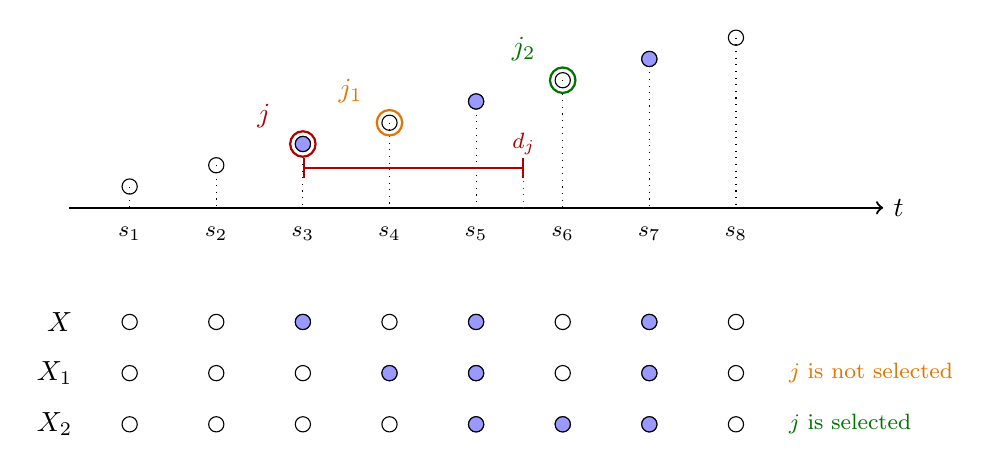
\begin{tikzpicture}[x=1.1cm,y=1cm]
\colorlet{prep}{red!70!black}
\colorlet{jone}{orange!90!black}
\colorlet{jtwo}{green!45!black}
\tikzset{dot/.style={draw,circle,inner sep=0pt,minimum size=5.5pt}}

% start times s_1, ..., s_8, in earliest-start-time order
\draw[->,thick] (0.3,0) -- (9.7,0) node[right] {$t$};
\foreach \i in {1,...,8}
{
    \pgfmathsetmacro{\yy}{0.27*\i}
    \draw[dotted] (\i,\yy) -- (\i,0);
    \node[font=\footnotesize] at (\i,-0.33) {$s_{\i}$};
    \node[dot] at (\i,\yy) {};
}
% the thresholds X = {3,5,7}; j = 3 is the smallest
\foreach \i in {3,5,7} \node[dot,fill=blue!40] at (\i,0.27*\i) {};
\draw[prep,thick] (3,0.27*3) circle (4.6pt);
\node[prep] at (2.55,0.27*3+0.35) {$j$};
% j_1 and j_2 are the smallest indices outside X above j, and with s >= d_j respectively
\draw[jone,thick] (4,0.27*4) circle (4.6pt);
\node[jone] at (3.55,0.27*4+0.4) {$j_1$};
\draw[jtwo,thick] (6,0.27*6) circle (4.6pt);
\node[jtwo] at (5.55,0.27*6+0.4) {$j_2$};
% the second operation of j
\draw[|-|,thick,prep] (3,0.27*3-0.3) -- (5.55,0.27*3-0.3);
\draw[dotted,prep] (5.55,0.27*3-0.3) -- (5.55,0);
\node[prep,font=\footnotesize] at (5.55,0.27*3+0.0) {$d_j$};

% the three threshold sets, one row each
\foreach \lab/\ysym/\members in {X/-1.45/{3,5,7}, X_1/-2.1/{4,5,7}, X_2/-2.75/{5,6,7}}
{
    \node[anchor=east] at (0.45,\ysym) {$\lab$};
    \foreach \i in {1,...,8} \node[dot] at (\i,\ysym) {};
    \foreach \i in \members \node[dot,fill=blue!40] at (\i,\ysym) {};
}
\node[anchor=west,font=\footnotesize,jone] at (8.5,-2.1) {$j$ is not selected};
\node[anchor=west,font=\footnotesize,jtwo] at (8.5,-2.75) {$j$ is selected};
\end{tikzpicture}
